\newpage
\subsubsection{Meccanismi di controllo e di rendicontazione}
	\paragraph{Meccanismi di controllo} Sono stati adottati dei meccanismi, nell'ambiente creato, per:
	\begin{itemize}
		\item Controllare l'andamento delle attività;
		\item Permettere un aggiornamento facilitato della pianificazione;
		\item Rendicontare le ore di lavoro spese nelle varie attività.
	\end{itemize}
	\paragraph{Controllo ritardi di attività}  Per mantenere il controllo sull'andamento generale si è scelto di adottare dei metodi grafici.
		\subparagraph{Dettaglio attività} Il sistema di ticketing adottato permette di visualizzare in modo dinamico il \textit{diagramma di  Gantt\ped{G}} delle attività. Viene visualizzato:
		\begin{itemize}
			\item La percentuale di completamento di ognuna di esse;
			\item Le attività in ritardo;
			\item Le attività concluse.
		\end{itemize}
		\begin{center}
			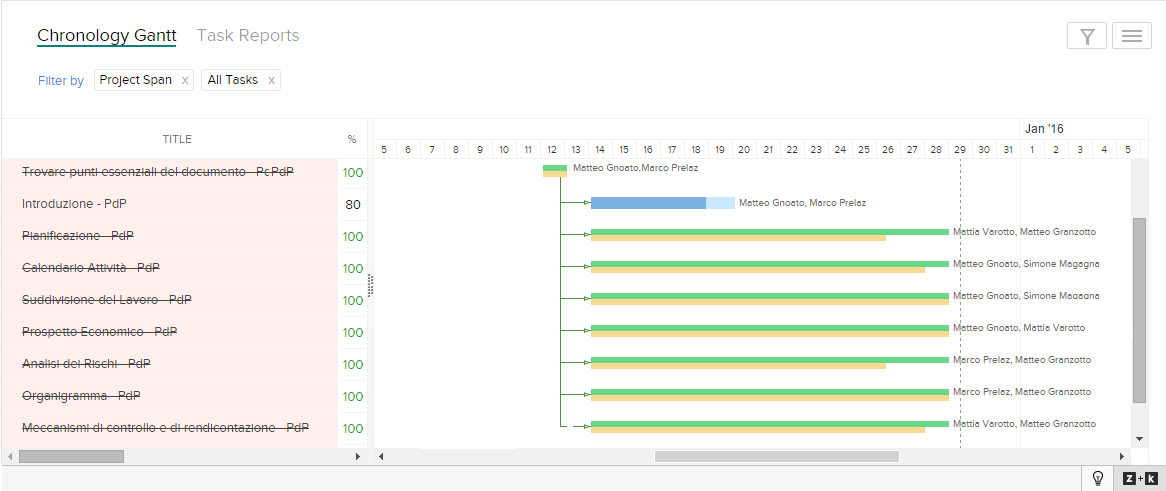
\includegraphics[keepaspectratio = true, width=16cm]{immagini/Norme_ZohoGantt.png}
		\end{center}
		\begin{figure}[h]
			\caption{\textit{Diagramma di Gantt\ped{G}} prodotto dal sistema di ticketing adottato}\label{etichetta}
		\end{figure}
		\subparagraph{Fasi processi}
		Combinando i dati del sistema di ticketing in un grafico ad area in pila per visualizzare il numero di ticket aperti in un particolare stato del \textit{ciclo di Deming\ped{G}}, è immediato visualizzare in quali stati si trovino le attività.
		\subparagraph{Controllo date} Per ottimizzare la pianificazione e tenerla in costante aggiornamento si utilizzano dei calendari a disposizione del gruppo.
		\subparagraph{Calendario attività}
		Il sistema di ticketing adottato genera automaticamente un calendario in cui vengono indicate inizio e fine delle varie attività.
		\subparagraph{Calendario risorse} Il calendario a disposizione del gruppo utilizzato per gestire il personale in base agli impegni dei vari componenti.
		\subparagraph{Controllo metriche di progetto} L'introduzione delle metriche consente di quantificare nel modo più obiettivo possibile le performance del gruppo nello svolgimento del progetto attraverso la misurazione dell'insieme di indicatori che ne fanno parte. Tipicamente uno degli usi più importanti delle metriche è quello di misurare l'avanzamento del progetto a fronte del piano. Il loro utilizzo consente di:
		\begin{itemize}
			\item Identificare i problemi di costo/schedulazione prima che diventino criticità;
			\item Aiutare il \textit{team\ped{G}} a focalizzarsi sul completamento delle proprie attività.
		\end{itemize}
		In particolare le metriche \textit{Budget Variance\ped{G}}(BV) e \textit{Schedule Variance\ped{G}}(SV) permettono rispettivamente di:
		\begin{itemize}
			\item Indicare se si è speso di più o di meno rispetto a quanto previsto;
			\item Indicare se si è in linea, in anticipo o in ritardo rispetto alla schedulazione delle	attività di progetto pianificate nella \textit{baseline\ped{G}}.
		\end{itemize}
		I valori aggiornati di tali metriche sono riportati nel \textit{\PdQ}.
	\paragraph{Meccanismi di rendicontazione} Il sistema di ticketing adottato mette a disposizione la rendicontazione delle ore di lavoro. Tale sistema permette di visualizzare le ore di lavoro in base all'attività svolta.
